\documentclass{article}
\usepackage[T1]{fontenc}
\usepackage[utf8]{inputenc}
\usepackage[spanish]{babel}
\usepackage[pdftex]{graphicx}
\usepackage{geometry}
\usepackage{caratula}

\begin{document}

\newgeometry{left=2cm,right=2cm}

\titulo{Trabajo Práctico 1A: \emph{Wiretapping}}
%\subtitulo{Subtítulo del tp}

%\fecha{\today}

\materia{Teoría de las Comunicaciones}
%\grupo{Grupo 42}

\integrante{Antonio, Pablo}{290/08}{pabloa@gmail.com}
\integrante{Ferrari, Gastón}{775/07}{gastonferrari5@hotmail.com}

\maketitle

\newgeometry{left=5cm,right=5cm}

\tableofcontents

\newpage

\section{Introducción}
El presente informe corresponde al Trabajo Práctico 1A, titulado
"\emph{Wiretapping}", de la materia Teoría de las Comunicaciones. El objetivo
de este trabajo es desarrollar una herramienta sencilla de diagnóstico de red
y realizar un análisis a partir de la información que esta nos provee en
distintos segmentos de red.

\section{Análisis de la entropía}
Para realizar este análisis, elegimos tres fuentes de información diferentes:

\begin{itemize}
    \item Fuente cuyos símbolos son IPs que realizan una consulta
        (\emph{request}) vía el protocolo ARP.
    \item Fuente cuyos símbolos son IPs que responden una consulta
        (\emph{reply}) vía el protocolo ARP.
    \item Fuente cuyos símbolos son IPs por las que se realiza una consulta
        (\emph{request}) vía el protocolo ARP.
\end{itemize}

Los datos fueron tomados de redes hogareñas.

\subsection{Red 1}
\subsubsection{Símbolos: IPs que realizan una consulta ARP}
La siguiente tabla muestra, para cada símbolo, su cantidad de apariciones y
sus medidas de probabilidad e información asociadas.

\vskip10pt

\begin{tabular}{|l|l|l|l|l|}
  \hline
  Símbolo & Apariciones & Probabilidad & Información \\
  \hline
  192.168.0.105 & 99 & $0.0947368421053$ & $3.39993060689$ \\
  \hline
  192.168.0.104 & 28 & $0.0267942583732$ & $5.22193230491$ \\
  \hline
  192.168.0.1 & 448 & $0.428708133971$ & $1.22193230491$ \\
  \hline
  192.168.0.101 & 415 & $0.397129186603$  & $1.33231970073$ \\
  \hline
  192.168.0.100 & 1 & $0.000956937799043$ & $10.029287227$ \\
  \hline
  192.168.0.103 & 11.0 & $0.0105263157895$ & $6.56985560833$ \\
  \hline
  192.168.0.102 & 26 & $0.0248803827751$ & $5.32884750883$ \\
  \hline
  0.0.0.0 & 17 & $0.0162679425837$ & $5.94182438572$ \\
  \hline
\end{tabular}

\vskip10pt

La entropía de la fuente es:

$$H(S) = 1.82297065237$$

En la figura \ref{fig:red1requesters:infoentro}, puede observarse gráficamente
los valores de información de cada símbolo en relación con la entropía de la
red.

\begin{figure}[h!]
    \centering                                                       
    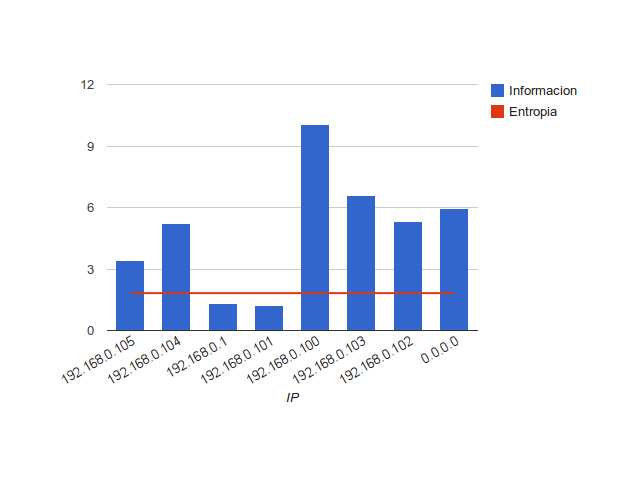
\includegraphics[width=300pt]{consultas1.png}
    \caption{Información de cada símbolo, en relación con la
        entropía de la red}
    \label{fig:red1requesters:infoentro}
\end{figure}

La figura \ref{fig:red1requesters:count} muestra la cantidad de apariciones de
cada símbolo. Podemos observar que las IPs 192.168.0.1 y 192.168.0.101 son las
que más pedidos realizan.

\begin{figure}[h!]
    \centering                                                       
    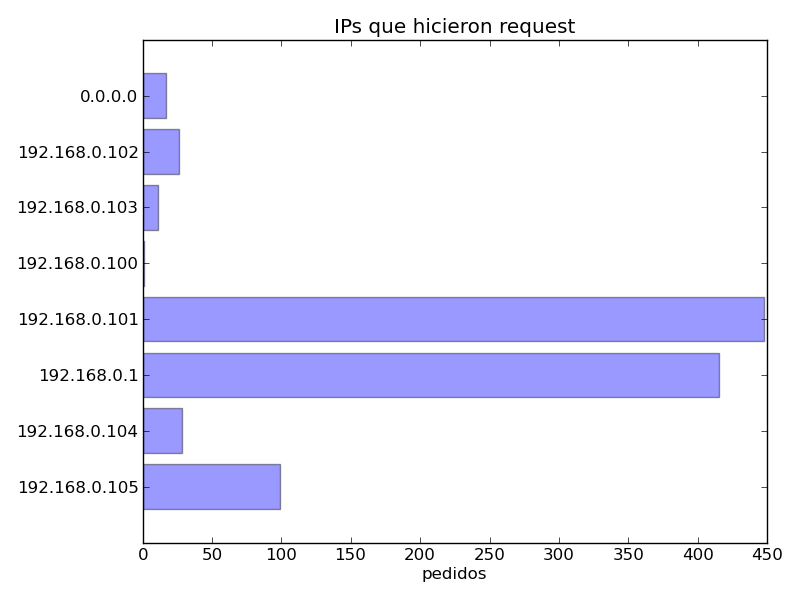
\includegraphics[width=300pt]{red1requesters.png}
    \caption{Apariciones de los símbolos}
    \label{fig:red1requesters:count}
\end{figure}

La figura \ref{fig:red1requesters:graph} permite observar qué IPs realizaron
consultas sobre qué otras IPs de la red. El tamaño de cada nodo se corresponde
con la cantidad de pedidos que realizó cada IP.

\begin{figure}[h!]
    \centering
    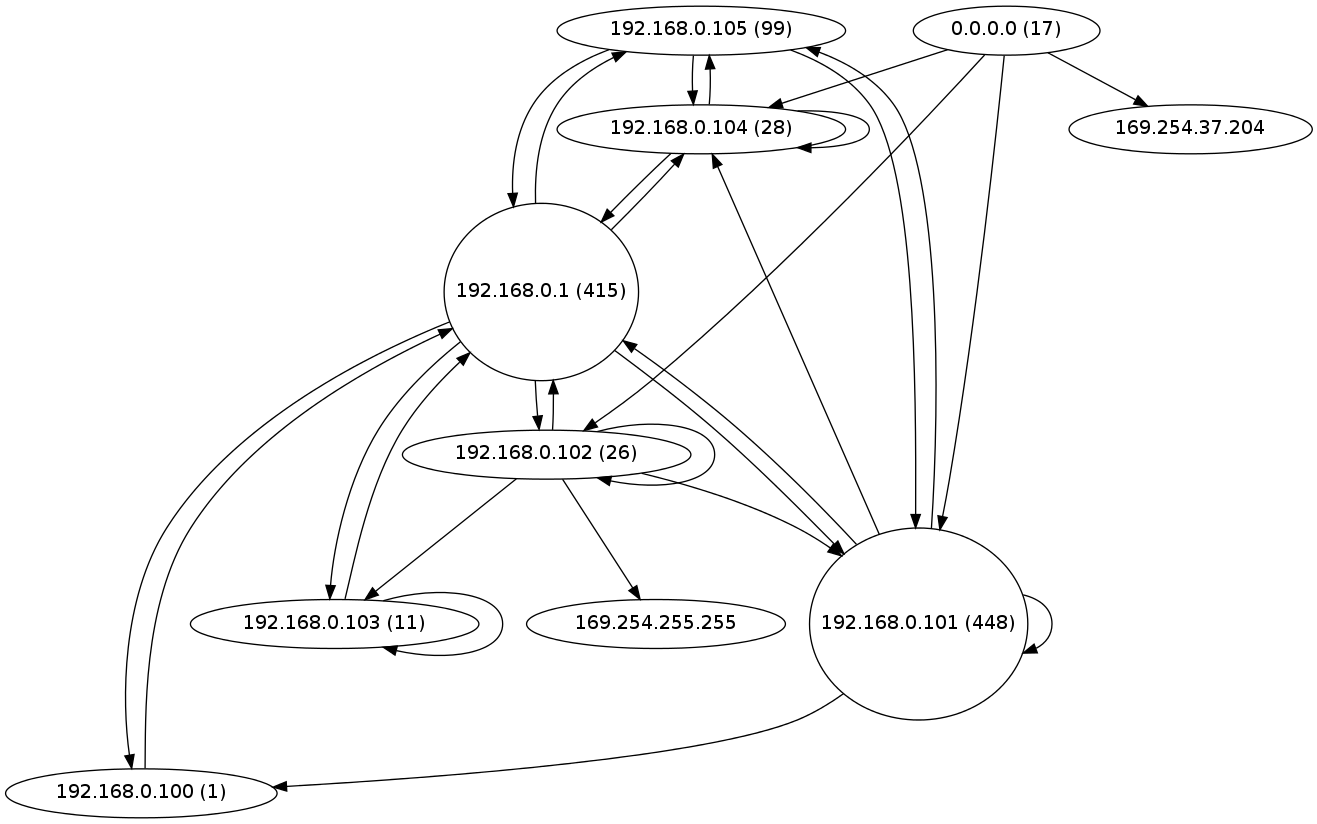
\includegraphics[width=350pt]{red1requestersgraph.png}
    \caption{Grafo en el que hay un eje desde una IP A a una IP B si la IP A
        realizó una consulta por la IP B}
    \label{fig:red1requesters:graph}
\end{figure}


% TODO: Esto estaba mal. Falta buscar una explicación a por qué aparece la
% 192.168.0.101.
%
%En este caso la IP que realiz\'o m\'as consultas ARP fue 192.168.0.1 (router),
%\'esto es l\'ogico considerando que el router es el encargado de distribuir
%todo el tr\'afico de la red a los nodos correspondientes por lo que su tabla
%de direcciones macs tiene que estar correctamente actualizada el mayor tiempo
%posible.\\\\


\subsubsection{Símbolos: IPs que responden una consulta ARP}
La siguiente tabla muestra, para cada símbolo, su cantidad de apariciones y
sus medidas de probabilidad e información asociadas.

\vskip10pt

\begin{tabular}{|l|l|l|l|l|}
  \hline
  Símbolo & Apariciones & Probabilidad & Información \\
  \hline
  192.168.0.105 & 506 & $0.85472972973$ & $0.226459790935$ \\
  \hline
  192.168.0.101 & 24 & $0.0405405405405$ & $4.62449086491$ \\
  \hline
  192.168.0.1 & 62 & $0.10472972973$ & $3.25525705524$ \\
  \hline
\end{tabular}\\

\vskip10pt

La entropía de la fuente es:

$$H(S) = 0.721963466885$$

En la figura \ref{fig:red1repliers:infoentro}, puede observarse gráficamente
los valores de información de cada símbolo en relación con la entropía de la
red.

\begin{figure}[h!]
    \centering                                                       
    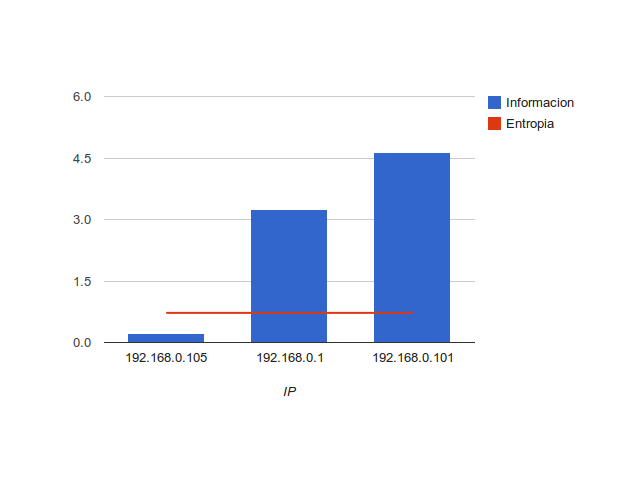
\includegraphics[width=300pt]{respuestas1.png}
    \caption{Información de cada símbolo, en relación con la
        entropía de la red}
    \label{fig:red1repliers:infoentro}
\end{figure}

La figura \ref{fig:red1repliers:count} muestra la cantidad de apariciones de
cada símbolo.

\begin{figure}[h!]
    \centering
    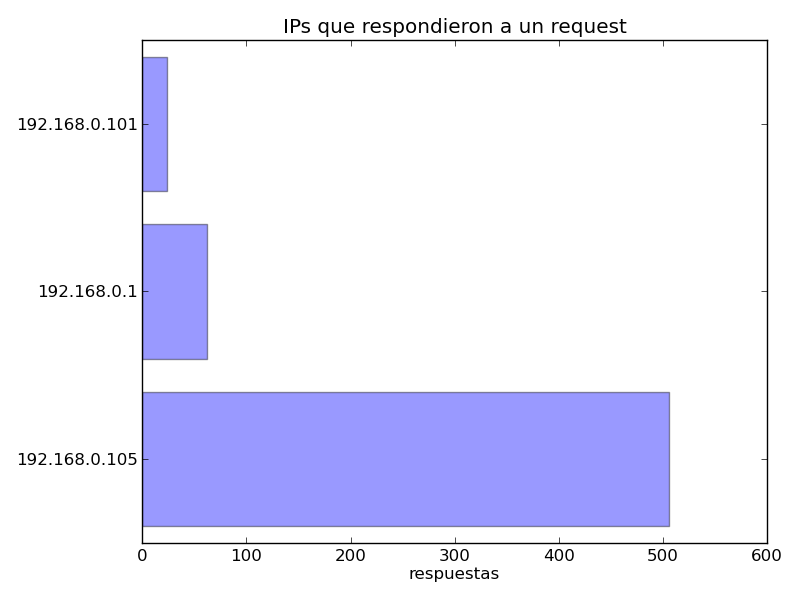
\includegraphics[width=300pt]{red1repliers.png}
    \caption{Apariciones de los símbolos}
    \label{fig:red1repliers:count}
\end{figure}

En este caso, la IP 192.168.0.105 fue la que más veces contestó los pedidos
sobre su dirección MAC; de ahí su probabilidad tan alta. Como se puede
observar, la información aportada por este símbolo es considerablemente más
baja que la aportada por los demás que poseen menor probabilidad. Incluso, la
información que representa es más baja que la entropía de la fuente.

\subsubsection{Símbolos: IPs por las que se realiza una consulta ARP}
La siguiente tabla muestra, para cada símbolo, su cantidad de apariciones y
sus medidas de probabilidad e información asociadas.

\vskip10pt

\begin{tabular}{|l|l|l|l|l|}
  \hline
  Símbolo & Consultas & Probabilidad & Información \\
  \hline
  169.254.37.204 & 3 & $0.00287081339713$ & $8.44432472625$\\
  \hline
  192.168.0.105 & 506 & $0.484210526316$ & $1.04629365227$\\
  \hline
  192.168.0.104 & 52 & $0.0497607655502$ & $4.32884750883$\\
  \hline
  169.254.255.255 & 10 & $0.00956937799043$ & $6.70735913208$\\
  \hline
  192.168.0.1 & 88 & $0.0842105263158$ & $3.56985560833$\\
  \hline
  192.168.0.101 & 30 & $0.0287081339713$ & $5.12239663136$\\
  \hline
  192.168.0.100 & 316 & $0.302392344498$ & $1.72550647879$\\
  \hline
  192.168.0.103 & 18 & $0.0172248803828$ & $5.85936222553$\\
  \hline
  192.168.0.102 & 22 & $0.0210526315789$ & $5.56985560833$\\
  \hline
\end{tabular}

\vskip10pt

La entropía de la fuente es:

$$H(S) = 1.99810125093$$

En la figura \ref{fig:red1requested:infoentro}, puede observarse gráficamente
los valores de información de cada símbolo en relación con la entropía de la
red.

\begin{figure}[h!]
    \centering                                                       
    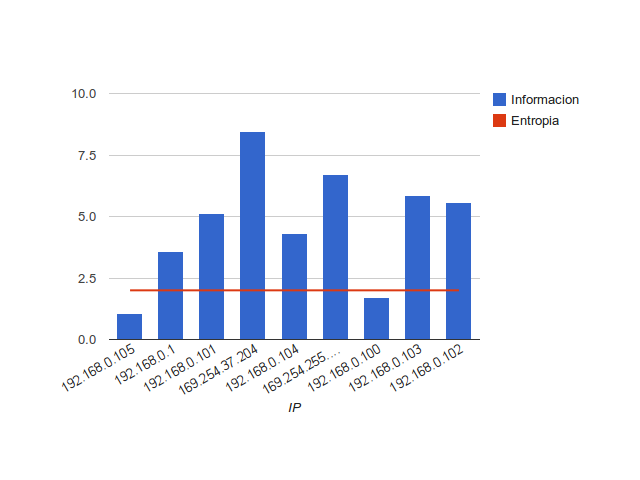
\includegraphics[width=300pt]{consultadas1.png}
    \caption{Información de cada símbolo, en relación con la
        entropía de la red}
    \label{fig:red1requested:infoentro}
\end{figure}

La figura \ref{fig:red1requested:count} muestra la cantidad de apariciones de
cada símbolo.

\begin{figure}[h!]
    \centering
    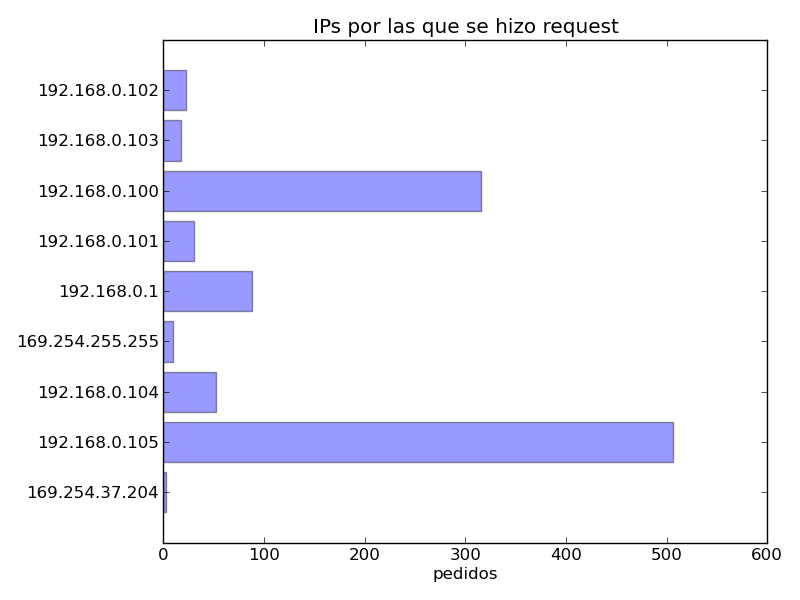
\includegraphics[width=300pt]{red1requested.png}
    \caption{Apariciones de los símbolos}
    \label{fig:red1requested:count}
\end{figure}

En este caso, la IP más consultada en la red fue la 192.168.0.105. Al igual
que en el punto anterior, por consecuencia de su alta probabilidad de aparecer
en la fuente, su información no supera a la entropía que ofrece la red.

\section{Conclusión}
A partir de los datos obtenidos se puede observar que hay más $requests$ que
$replys$, ésto se debe entre otras cosas a que los hosts hacen consultas por
su propia IP para asegurarse que no haya otro host con ésa dirección en la
red. A su vez puede haber consultas que no son respondidas y paquetes que se
pierden.\\ Nos resultó extraño que apareciera como IP fuente de algunos
pedidos la IP 0.0.0.0 pero investigando un poco nos dimos cuenta que ésto
sucede cuando un host se conecta a la red y se hace para verificar que no haya
otro host con la misma IP.\\ El protocolo ARP no es seguro ya que permite que
un host se haga pasar por otro, respondiendo mensajes ARP que no estaban
dirigidos a él. Ésto se conoce como ARP Spoofing.

\end{document}
